% =====================================================================
%  Prerequisites: laws for sine and cosine
%  Requires in preamble.tex:
%    \usepackage{amsthm}
%    \newtheorem{lemma}{Lemma}[chapter]
% =====================================================================
\chapter{Prerequisites}

The book Mathematik~\cite{arens2015} can be used to study all the math required for this project.


% =====================================================================
%  Fundamentale physikalische Größen
%  Requires in preamble.tex:  \usepackage[ngerman, english]{babel}
% =====================================================================

\begin{otherlanguage}{ngerman}

\section{Fundamentale physikalische Größen}
\label{sec:physical-quantities}

\paragraph{1.\ Impuls.}
\[
  \vect{p} = m \vect{v}
\]

\paragraph{2.\ Kraft.}
\[
  \vect{F} = \frac{d\vect{p}}{dt} , \qquad
  \vect{F} = m \vect{a}
\]

\paragraph{3.\ Drehimpuls.}
\[
  \vect{L} = \vect{r} \times \vect{p}
           = m \, \vect{r} \times \vect{v}
           = m \, (\vect{r} \cdot \vect{r}) \, \vect{\omega} ,
  \qquad \text{unter der Annahme } \langle \vect{r}, \vect{\omega} \rangle = 0 .
\]
Der Drehimpuls hängt von der Wahl des Bezugspunktes ab. Meint man
allerdings den Drehimpuls eines Körpers, ist dieser Bezugspunkt eindeutig
als der Schwerpunkt festgelegt.

\paragraph{4.\ Drehmoment.}
\[
  \vect{M} = \frac{d\vect{L}}{dt} , \qquad
  \vect{M} = \vect{r} \times \vect{F}
\]
Das Drehmoment verhält sich zum Drehimpuls wie die Kraft zum Impuls.

\paragraph{5.\ Trägheitsmoment.}
Das Trägheitsmoment ist definiert als eine Größe, die natürlich in den
Formeln für kinetische Energie, Drehimpuls und Drehmoment auftritt. Hier
werden die Größen für eine Scheibe beschrieben, die in der
$x$-$y$-Ebene liegt und sich um die $z$-Achse dreht. $r$ gibt dabei den
Abstand zur $z$-Achse an und $\rho$ die Flächendichte.
% Added during transcription -- please check.
$\omega$ und $\alpha$ sind die Winkelgeschwindigkeit und die
Winkelbeschleunigung der Scheibe, $v(r) = \omega r$ und $a(r) = \alpha r$
die Bahngeschwindigkeit und die Bahnbeschleunigung im Abstand $r$, und
\[
  I = \iint \rho(r,\varphi) \, r^2 \, r \, dr \, d\varphi .
\]
Damit gilt
\begin{align*}
  L &= \iint \rho(r,\varphi) \, v(r) \, r \; r \, dr \, d\varphi
     = \iint \rho(r,\varphi) \, \omega r^2 \; r \, dr \, d\varphi
     = \omega I , \\
  E_\text{kin} &= \frac{1}{2} \iint \rho(r,\varphi) \, v(r)^2 \; r \, dr \, d\varphi
     = \frac{1}{2} \iint \rho(r,\varphi) \, \omega^2 r^2 \; r \, dr \, d\varphi
     = \frac{1}{2} \omega^2 I , \\
  M &= \iint \rho(r,\varphi) \, a(r) \, r \; r \, dr \, d\varphi
     = \iint \rho(r,\varphi) \, \alpha r^2 \; r \, dr \, d\varphi
     = \alpha I .
\end{align*}
Diese Beschreibungen sind allgemein und hilfreich für nicht deformierbare
Scheiben. Das Trägheitsmoment nimmt eine ähnliche Rolle ein wie die Masse.

\end{otherlanguage}

\section{Laws for sine and cosine}
\label{sec:triangle-laws}

\begin{lemma}[Laws for sine and cosine]
\label{lem:triangle-laws}
Let $a$ and $c$ be the lengths of the edges adjacent to the angle $\alpha$
of a triangle, and let $b$ be the length of the edge opposite to $\alpha$.
Then
\begin{align}
  \cos(\alpha) &= \frac{a^2 + c^2 - b^2}{2ac}, \label{eq:law-of-cosines} \\
  \sin(\alpha) &= \frac{1}{2ac}
    \sqrt{(a+c+b)(a+c-b)(a-c+b)(a-c-b)}. \label{eq:sine-from-sides}
\end{align}
% TODO: check the sign of the radicand in \eqref{eq:sine-from-sides}.
\end{lemma}

\begin{proof}
\emph{Cosine.}
If $\alpha$ is acute (\cref{fig:triangle-acute}), the altitude onto the
edge $a$ has length $c\sin(\alpha)$ and divides $a$ into two segments, so
that

\begin{figure}[tbp]
  \centering
  \begin{tikzpicture}[scale=1.1, thick]
    % vertices: A has angle alpha; a and c leave A, b is opposite
    \coordinate (A)  at (0,0);
    \coordinate (Pa) at (5,0);
    \coordinate (Pc) at ({3.5*cos(55)},{3.5*sin(55)});
    \coordinate (F)  at ({3.5*cos(55)},0);
    % triangle
    \draw (A) -- node[pos=0.85, above] {$a$} (Pa)
              -- node[above right] {$b$} (Pc)
              -- node[above left] {$c$} cycle;
    % altitude
    \draw[dashed] (Pc) -- node[left, pos=0.75] {$c\sin(\alpha)$} (F);
    \pic[draw, angle radius=6pt] {right angle = Pa--F--Pc};
    % angle
    \pic[draw, "$\alpha$", angle radius=18pt, angle eccentricity=1.45]
      {angle = Pa--A--Pc};
    % segments of a
    \draw[|<->|, thin] ($(A)+(0,-0.3)$) -- node[below, font=\small]
      {$c\cos(\alpha)$} ($(F)+(0,-0.3)$);
    \draw[|<->|, thin] ($(F)+(0,-0.3)$) -- node[below, font=\small]
      {$\sqrt{b^2 - c^2\sin^2(\alpha)}$} ($(Pa)+(0,-0.3)$);
  \end{tikzpicture}
  \caption{Triangle with acute angle $\alpha$. The altitude onto $a$
    divides $a$ into two segments.}
  \label{fig:triangle-acute}
\end{figure}
\begin{align*}
  a &= c\cos(\alpha) + \sqrt{b^2 - c^2\sin^2(\alpha)} \\
  \Rightarrow\quad
  a^2 - 2ac\cos(\alpha) + c^2\cos^2(\alpha) &= b^2 - c^2\sin^2(\alpha) \\
  \Rightarrow\quad
  a^2 - 2ac\cos(\alpha) &= b^2 - c^2 \\
  \Rightarrow\quad
  \cos(\alpha) &= \frac{a^2 + c^2 - b^2}{2ac}.
\end{align*}
If $\alpha$ is obtuse (\cref{fig:triangle-obtuse}), the altitude falls
outside the triangle, onto the extension of the edge $c$, and has length
$a\sin(\pi-\alpha)$. Then

\begin{figure}[tbp]
  \centering
  \begin{tikzpicture}[scale=1.1, thick]
    \coordinate (A)  at (0,0);
    \coordinate (Pc) at (5,0);
    \coordinate (Pa) at ({2.8*cos(125)},{2.8*sin(125)});
    \coordinate (F)  at ({2.8*cos(125)},0);
    % triangle
    \draw (A) -- node[below] {$c$} (Pc)
              -- node[above right] {$b$} (Pa)
              -- node[above right] {$a$} cycle;
    % extension of c and altitude
    \draw[dashed] (A) -- (F);
    \draw[dashed] (Pa) -- node[left] {$a\sin(\pi-\alpha)$} (F);
    \pic[draw, angle radius=6pt] {right angle = A--F--Pa};
    % angles
    \pic[draw, "$\alpha$", angle radius=10pt, angle eccentricity=1.7]
      {angle = Pc--A--Pa};
    \pic[draw, "$\pi-\alpha$", angle radius=16pt, angle eccentricity=2.1]
      {angle = Pa--A--F};
    % segment on the extended line
    \draw[|<->|, thin] ($(F)+(0,-0.6)$) -- node[below, font=\small]
      {$\sqrt{b^2 - a^2\sin^2(\pi-\alpha)}$} ($(Pc)+(0,-0.6)$);
  \end{tikzpicture}
  \caption{Triangle with obtuse angle $\alpha$. The altitude falls onto
    the extension of $c$.}
  \label{fig:triangle-obtuse}
\end{figure}
\begin{align*}
  c &= \sqrt{b^2 - a^2\sin^2(\pi-\alpha)} - a\cos(\pi-\alpha) \\
    &= \sqrt{b^2 - a^2\sin^2(\alpha)} + a\cos(\alpha) \\
  \Rightarrow\quad
  c^2 - 2ac\cos(\alpha) + a^2\cos^2(\alpha) &= b^2 - a^2\sin^2(\alpha) \\
  \Rightarrow\quad
  c^2 - 2ac\cos(\alpha) &= b^2 - a^2 \\
  \Rightarrow\quad
  \cos(\alpha) &= \frac{a^2 + c^2 - b^2}{2ac}.
\end{align*}
In general this holds for any of the three angles of the triangle: the
lengths that can be interchanged without changing the result are always
those of the two adjacent edges, and the remaining length is that of the
opposite edge.

\emph{Sine.}
Using \eqref{eq:law-of-cosines},
\begin{align*}
  \sin(\alpha)
  &= \sqrt{1 - \cos^2(\alpha)}
   = \sqrt{\bigl(1 + \cos(\alpha)\bigr)\bigl(1 - \cos(\alpha)\bigr)} \\
  &= \sqrt{\left(1 + \frac{a^2 + c^2 - b^2}{2ac}\right)
           \left(1 - \frac{a^2 + c^2 - b^2}{2ac}\right)} \\
  &= \sqrt{\left(\frac{(a+c)^2 - b^2}{2ac}\right)
           \left(\frac{(a-c)^2 - b^2}{2ac}\right)} \\
  &= \frac{1}{2ac}\sqrt{(a+c+b)(a+c-b)(a-c+b)(a-c-b)}.
\end{align*}
\end{proof}

% =====================================================================
%  Curvature
%  Requires: \cite{wiki-curvature} in references.bib
% =====================================================================

\section{Curvature}
\label{sec:curvature}

This section on curvature closely follows Wikipedia~\cite{wiki-curvature}.

\paragraph{Definition.}
\begin{equation}
  \kappa = \left\lVert \frac{d\vect{T}}{ds} \right\rVert ,
  \label{eq:curvature-def}
\end{equation}
where $s$ denotes the arc length and $\vect{T}$ the normalized tangent
vector,
\[
  \lVert \vect{T} \rVert = 1 \quad \text{for all } s \in [0, L] ,
\]
where $L$ describes the length of the curve or the length at which the
curve repeats ($2\pi r$ for a circle with radius $r$).

Since every tangent vector is normalized, we can express it in the form
\[
  \vect{T}(s) = \begin{pmatrix} \cos(\varphi(s)) \\ \sin(\varphi(s)) \end{pmatrix} ,
\]
% Added during transcription -- please check.
where $\varphi(s)$ is the angle of the tangent vector.
Therefore we find
\[
  \kappa
  = \left\lVert \frac{d\vect{T}(s)}{ds} \right\rVert
  = \left\lVert \begin{pmatrix} -\sin(\varphi(s)) \\ \cos(\varphi(s)) \end{pmatrix}
    \frac{d\varphi(s)}{ds} \right\rVert
  = |\frac{d\varphi}{ds}| .
\]

If a curve $\vect{\gamma}(t)$ is not parametrized in terms of the arc
length, we can find its arc-length parametrization
$\bar{\vect{\gamma}}(s)$ via
\[
  s(t) = \int_0^t dt \, \lVert \dot{\vect{\gamma}}(t) \rVert
\]
and therefore
\[
  \frac{ds}{dt} = \lVert \dot{\vect{\gamma}}(t) \rVert
  \quad\text{and}\quad
  \frac{dt}{ds} = \frac{1}{\lVert \dot{\vect{\gamma}}(t) \rVert} .
\]
With those we find
\[
  \frac{d\bar{\vect{\gamma}}(s)}{ds}
  = \frac{d\vect{\gamma}(t(s))}{ds}
  = \frac{\partial \vect{\gamma}}{\partial t} \frac{dt}{ds}
  = \dot{\vect{\gamma}}(t) \frac{1}{\lVert \dot{\vect{\gamma}}(t) \rVert} .
\]
Since $d\bar{\vect{\gamma}}/ds$ is the tangent vector, we can also
immediately verify the normalization of the tangent vector.

One can also use the chain rule again to find the curvature in the
non-arc-length parametrization:
\[
  \kappa = \left\lVert \frac{d\vect{T}}{ds} \right\rVert
\]
with
\begin{align*}
  \frac{d\vect{T}}{ds}
  &= \frac{d}{ds} \left( \frac{\dot{\vect{\gamma}}(t(s))}
                              {\lVert \dot{\vect{\gamma}}(t(s)) \rVert} \right) \\
  &= \frac{\ddot{\vect{\gamma}}(t(s))}{\lVert \dot{\vect{\gamma}}(t) \rVert}
     \cdot \frac{1}{\lVert \dot{\vect{\gamma}}(t) \rVert}
   - \frac{1}{2}
     \frac{\dot{\vect{\gamma}}(t)}
          {\bigl(\dot{\vect{\gamma}}(t) \cdot \dot{\vect{\gamma}}(t)\bigr)^{3/2}}
     \cdot 2 \, \dot{\vect{\gamma}}(t) \cdot \ddot{\vect{\gamma}}(t)
     \cdot \frac{1}{\lVert \dot{\vect{\gamma}}(t) \rVert} \\
  &= \frac{\ddot{\vect{\gamma}}(t)}{\lVert \dot{\vect{\gamma}}(t) \rVert^2}
   - \dot{\vect{\gamma}}(t)
     \bigl(\dot{\vect{\gamma}}(t) \cdot \ddot{\vect{\gamma}}(t)\bigr)
     \frac{1}{\lVert \dot{\vect{\gamma}}(t) \rVert^4} \\
  &= \frac{\ddot{\vect{\gamma}}(t)}{\lVert \dot{\vect{\gamma}}(t) \rVert^2}
   - \vect{T} \bigl(\vect{T} \cdot \ddot{\vect{\gamma}}(t)\bigr)
     \frac{1}{\lVert \dot{\vect{\gamma}}(t) \rVert^2} .
\end{align*}
Therefore
\begin{align}
  \kappa = \left\lVert \frac{d\vect{T}}{ds} \right\rVert
  &= \sqrt{ \frac{\lVert \ddot{\vect{\gamma}}(t) \rVert^2}
                 {\lVert \dot{\vect{\gamma}}(t) \rVert^4}
          + \frac{\bigl(\vect{T} \cdot \ddot{\vect{\gamma}}(t)\bigr)^2}
                 {\lVert \dot{\vect{\gamma}}(t) \rVert^4}
          - 2 \, \frac{\bigl(\vect{T} \cdot \ddot{\vect{\gamma}}(t)\bigr)^2}
                      {\lVert \dot{\vect{\gamma}}(t) \rVert^4} }
  \notag \\
  &= \sqrt{ \frac{\lVert \ddot{\vect{\gamma}}(t) \rVert^2
                  \lVert \dot{\vect{\gamma}}(t) \rVert^2}
                 {\lVert \dot{\vect{\gamma}}(t) \rVert^6}
          - \frac{\bigl(\dot{\vect{\gamma}}(t) \cdot \ddot{\vect{\gamma}}(t)\bigr)^2}
                 {\lVert \dot{\vect{\gamma}}(t) \rVert^6} }
  \notag \\
  &= \frac{\sqrt{ \lVert \ddot{\vect{\gamma}}(t) \rVert^2
                  \lVert \dot{\vect{\gamma}}(t) \rVert^2
                - \bigl(\dot{\vect{\gamma}}(t) \cdot \ddot{\vect{\gamma}}(t)\bigr)^2 }}
          {\lVert \dot{\vect{\gamma}}(t) \rVert^3} .
  \label{eq:curvature-general}
\end{align}

\subsection{Special curvatures}
\label{sec:curvature-special}

\paragraph{1.\ Circle.}
A circle is typically parametrized by the angle $\theta$:
\[
  \vect{\gamma}(\theta) =
  \begin{pmatrix} r\cos(\theta) \\ r\sin(\theta) \end{pmatrix} .
\]
Its arc length is
\[
  s(\theta) = \int_0^\theta d\theta \,
  \left\lVert \begin{pmatrix} -r\sin(\theta) \\ r\cos(\theta) \end{pmatrix} \right\rVert
  = r\theta ,
  \qquad\text{so}\qquad
  \theta(s) = \frac{s}{r} ,
\]
and we find the curve parametrized with the arc length $s$:
\[
  \vect{\gamma}(\theta(s)) =
  \begin{pmatrix} r\cos\left(\frac{s}{r}\right) \\ r\sin\left(\frac{s}{r}\right) \end{pmatrix} ,
  \qquad
  \vect{T} = \frac{d\vect{\gamma}}{ds} =
  \begin{pmatrix} -\sin\left(\frac{s}{r}\right) \\ \cos\left(\frac{s}{r}\right) \end{pmatrix} ,
  \qquad
  \frac{d\vect{T}}{ds} =
  \begin{pmatrix} -\frac{1}{r}\cos\left(\frac{s}{r}\right) \\
                  -\frac{1}{r}\sin\left(\frac{s}{r}\right) \end{pmatrix} ,
\]
and therefore the curvature
\[
  \kappa(s) = \left\lVert \frac{d\vect{T}(s)}{ds} \right\rVert = \frac{1}{r} .
\]

\paragraph{2.\ Graph of a function.}
% "dots denote derivatives with respect to x" added during transcription.
For the graph of a function $f$, where dots denote derivatives with
respect to $x$,
\[
  \vect{\gamma}(x) = \begin{pmatrix} x \\ f(x) \end{pmatrix} ,
  \qquad
  \dot{\vect{\gamma}}(x) = \begin{pmatrix} 1 \\ \dot{f}(x) \end{pmatrix} ,
  \qquad
  \ddot{\vect{\gamma}}(x) = \begin{pmatrix} 0 \\ \ddot{f}(x) \end{pmatrix} .
\]
Now we can use the general parametrization formula
\eqref{eq:curvature-general}:
\begin{align*}
  \kappa &= \frac{\sqrt{ \bigl(\ddot{f}(x)\bigr)^2 \bigl(1 + (\dot{f}(x))^2\bigr)
                       - \bigl(\dot{f}(x)\,\ddot{f}(x)\bigr)^2 }}
                 {\bigl(1 + (\dot{f}(x))^2\bigr)^{3/2}} , \\
  \kappa &= \frac{|\ddot{f}(x)|}{\bigl(1 + (\dot{f}(x))^2\bigr)^{3/2}} .
\end{align*}

\paragraph{3.\ Generalization of a circle.}
% "dots denote derivatives with respect to theta" added during transcription.
With a radius $r(\theta)$ that depends on the angle, where dots denote
derivatives with respect to $\theta$ and the argument $\theta$ of the
trigonometric functions is omitted on the right,
\begin{align*}
  \vect{\gamma}(\theta) &=
  \begin{pmatrix} r(\theta)\cos(\theta) \\ r(\theta)\sin(\theta) \end{pmatrix} , \\
  \dot{\vect{\gamma}}(\theta) &=
  \begin{pmatrix} \dot{r}\cos - r\sin \\ \dot{r}\sin + r\cos \end{pmatrix} , \\
  \ddot{\vect{\gamma}}(\theta) &=
  \begin{pmatrix} \ddot{r}\cos - 2\dot{r}\sin - r\cos \\
                  \ddot{r}\sin + 2\dot{r}\cos - r\sin \end{pmatrix} ,
\end{align*}
with
\begin{align*}
  \lVert \dot{\vect{\gamma}}(\theta) \rVert^2 &= \dot{r}^2 + r^2 , \\
  \lVert \ddot{\vect{\gamma}}(\theta) \rVert^2 &=
    \ddot{r}^2 + r^2 + 4\dot{r}^2 - 2\ddot{r}r , \\
  \bigl(\dot{\vect{\gamma}} \cdot \ddot{\vect{\gamma}}\bigr) &=
    \ddot{r}\dot{r} + r\dot{r} .
\end{align*}
We find
\begin{align*}
  \lVert \dot{\vect{\gamma}}(\theta) \rVert^2
  \lVert \ddot{\vect{\gamma}}(\theta) \rVert^2
  &= \ddot{r}^2\dot{r}^2 + 4\dot{r}^4 + r^2\dot{r}^2 - 2r\ddot{r}\dot{r}^2
   + r^2\ddot{r}^2 + 4\dot{r}^2r^2 + r^4 - 2r^3\ddot{r} , \\
  \bigl(\dot{\vect{\gamma}} \cdot \ddot{\vect{\gamma}}\bigr)^2
  &= \ddot{r}^2\dot{r}^2 + 2\ddot{r}\dot{r}^2 r + r^2\dot{r}^2 , \\
  \lVert \dot{\vect{\gamma}}(\theta) \rVert^2
  \lVert \ddot{\vect{\gamma}}(\theta) \rVert^2
  - \bigl(\dot{\vect{\gamma}}(\theta) \cdot \ddot{\vect{\gamma}}(\theta)\bigr)^2
  &= 4\dot{r}^4 - 4\ddot{r}\dot{r}^2 r + r^2\ddot{r}^2
   + 4\dot{r}^2r^2 + r^4 - 2r^3\ddot{r} \\
  &= \bigl(r^2 + 2\dot{r}^2 - r\ddot{r}\bigr)^2 ,
\end{align*}
so we find
\[
  \kappa
  = \frac{\sqrt{ \lVert \dot{\vect{\gamma}}(\theta) \rVert^2
                 \lVert \ddot{\vect{\gamma}}(\theta) \rVert^2
               - \bigl(\dot{\vect{\gamma}}(\theta) \cdot \ddot{\vect{\gamma}}(\theta)\bigr)^2 }}
         {\lVert \dot{\vect{\gamma}}(\theta) \rVert^3}
  = \frac{r^2 + 2\dot{r}^2 - r\ddot{r}}{\bigl(r^2 + \dot{r}^2\bigr)^{3/2}} .
\]

% =====================================================================
%  Lineare Balkentheorie
%  Requires in preamble.tex:  \usepackage[ngerman, english]{babel}
%  (english stays the main language because it is loaded last)
%  Requires: tikz (calc, angles, quotes, patterns)
% =====================================================================

% =====================================================================
%  Lineare Balkentheorie
%  Requires in preamble.tex:  \usepackage[ngerman, english]{babel}
%  (english stays the main language because it is loaded last)
%  Requires: tikz (calc, angles, quotes, patterns)
% =====================================================================

\begin{otherlanguage}{ngerman}

\section{Lineare Balkentheorie}
\label{sec:beam-theory}

Die alleinige Quelle für diesen Abschnitt ist das Buch TM 2 by Gross \cite{gross2024tm2}.
Wer mehr als nur eine kurze Aufffrischung braucht sollte das Kapitel zur Balkenbiegung 
zu Rate ziehen. Dort sind die Zusammenhänge auch sicherlich besser dargestellt und mehr 
Aufwand ist in die einwandfreie Visualisierung der Inhalte geflossen. 

\paragraph{Motivation.}
Wir wollen sicherstellen, dass sich der Arm nur minimal unter seiner
eigenen Last und dem zu hebenden Gewicht verformt. Da wir somit sehr
kleine Verformungen voraussetzen, ist die lineare Balkentheorie
ausreichend. Eine mögliche Schlussfolgerung aus konkreten Berechnungen
kann allerdings sein, dass die maximal zulässige Last für eine bestimmte
kleine Verformung im realistischen Betrieb überschritten wird. Möchte man
dennoch weder die Konstruktion des Arms noch die zulässige Last anpassen,
muss man die Verformungen in höheren Ordnungen entwickeln und dann die
Position des Arms entsprechend der Verformung korrigieren. Letzteres ist
allerdings sicherlich ein schwieriges Unterfangen und man wäre wohl besser
beraten, wo möglich die Konstruktion anzupassen.

\paragraph{Szenario.}
\begin{center}
% Deformation strongly exaggerated. The deflection curve is the solution
% w(s) derived at the end of this section, scaled to w(L) = 0.6.
\begin{tikzpicture}[thick, scale=1.6,
  declare function={
    wd(\x) = 0.6*\x*\x*(12-\x)/128;      % deflection
    wp(\x) = 0.6*3*\x*(8-\x)/128;        % slope dw/ds
    nn(\x) = sqrt(1+wp(\x)^2);
  }]
  % clamped wall
  \fill[pattern=north east lines] (-0.25,-1.0) rectangle (0,0.8);
  \draw (0,-1.0) -- (0,0.8);
  % undeformed beam (reference)
  \draw[thin, gray, densely dotted] (0,-0.4) rectangle (4,0.4);
  % deformed beam: edges offset by the half height along the normal
  \draw plot[domain=0:4, samples=40, smooth]
    ({\x + 0.4*wp(\x)/nn(\x)}, {-wd(\x) + 0.4/nn(\x)});
  \draw plot[domain=0:4, samples=40, smooth]
    ({\x - 0.4*wp(\x)/nn(\x)}, {-wd(\x) - 0.4/nn(\x)});
  \draw ({4 + 0.4*wp(4)/nn(4)}, {-wd(4) + 0.4/nn(4)})
     -- ({4 - 0.4*wp(4)/nn(4)}, {-wd(4) - 0.4/nn(4)});
  % neutral line
  \draw[dashed, thin] plot[domain=0:4, samples=40, smooth] (\x, {-wd(\x)});
  % local axes
  \draw[-{Stealth[length=4pt]}, semithick, blue!70!black]
    (0,0) -- (0.6,0) node[above] {$x$};
  \draw[-{Stealth[length=4pt]}, semithick, blue!70!black]
    (0.02,0) -- (0.02,0.65) node[right] {$z$};
  % cross-section at s = 3, perpendicular to the deformed neutral line
  \pgfmathsetmacro{\psideg}{atan(wp(3))}
  \coordinate (C) at (3, {-wd(3)});
  \draw[dashed, thin] ($(C)+(0,-0.6)$) -- ($(C)+(0,1.05)$) coordinate (V);
  \draw ($(C)+(270-\psideg:0.6)$) -- ($(C)+(90-\psideg:1.0)$) coordinate (S);
  \pic[draw, thin, "$\psi$", angle radius=34pt, angle eccentricity=1.3]
    {angle = S--C--V};
  % force at the deformed end
  \coordinate (Ft) at ({4 + 0.4*wp(4)/nn(4)}, {-wd(4) + 0.4/nn(4)});
  \draw[-{Stealth[length=6pt]}] ($(Ft)+(0,1.1)$) -- node[right] {$F$} (Ft);
\end{tikzpicture}
\end{center}

Die Deformation des Balkens ist hier zu Gunsten der Anschaulichkeit übertrieben 
dargestellt.
\emph{Annahme:} Die mittlere gestrichelte Linie beschreibt die Linie,
welche ihre Länge als Konsequenz der Verformung nicht verändert. $u$
beschreibt die Verschiebung parallel zu dieser Linie, $w$ beschreibt die
Verschiebung vertikal zu $u(s,t)$, aber immer noch in der skizzierten
Ebene liegend.

Da wir sehr kleine Verformungen annehmen, sind die $s$- und $t$-Achse
beinahe parallel zu jeweils der $x$- und $z$-Achse.

Betrachten wir nun den skizzierten Querschnitt an Stelle $s$:
\begin{center}
\begin{tikzpicture}[thick, scale=1.6]
  \coordinate (O) at (0,0);
  \coordinate (V) at (0,1.1);
  \draw[-{Stealth[length=4pt]}, semithick] (O) -- (0.9,0) node[right] {$x$};
  \draw[-{Stealth[length=4pt]}, semithick] (0,-1.1) -- (V) node[left] {$z$};
  % rotated cross-section: top shifted by u to the right
  \draw (-0.36,-1) -- (0.36,1) coordinate (S);
  \pic[draw, thin, "$\psi$", angle radius=16pt, angle eccentricity=1.4]
    {angle = S--O--V};
  % u at the top
  \draw[|<->|, thin] (0,1.3) -- node[above] {$u$} (0.36,1.3);
\end{tikzpicture}
\end{center}
Dann gilt offensichtlich
\[
  \psi(s) = \arctan\left(\frac{u}{z}\right) .
\]
Da wir annehmen, dass $\psi(s)$ sehr klein ist, muss auch $u/z$ sehr klein
sein:
\[
  \psi(s) \approx \frac{u}{z} ,
\]
\begin{equation}
  \boxed{u(s,z) = \psi(s)\, z}
  \label{eq:beam-u}
\end{equation}

Betrachten wir nun ein infinitesimales Element und stellen uns vor, dass
dieses Element aus horizontal gekoppelten Federn besteht:
\begin{center}
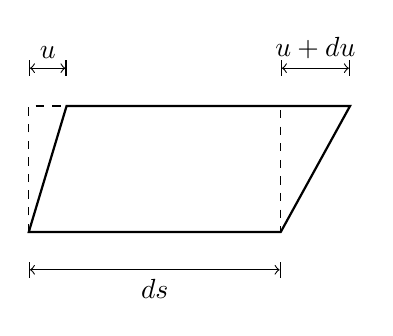
\begin{tikzpicture}[thick, scale=1.6]
  \draw[dashed, thin] (0,0) rectangle (2,1);
  \draw (0,0) -- (2,0) -- (2.55,1) -- (0.3,1) -- cycle;
  \draw[|<->|, thin] (0,1.3) -- node[above] {$u$} (0.3,1.3);
  \draw[|<->|, thin] (2,1.3) -- node[above] {$u + du$} (2.55,1.3);
  \draw[|<->|, thin] (0,-0.3) -- node[below] {$ds$} (2,-0.3);
\end{tikzpicture}
\end{center}
Dann beschreibt $du(z)$ genau die Streckung bzw.\ Stauchung dieser Federn
und $\frac{du}{ds}(s,z)$ beschreibt die Stauchung durch die Länge $ds$ der
entspannten Feder.

Es lässt sich experimentell das Elastizitätsmodul $E$ bestimmen:
\begin{equation}
  \boxed{\sigma = E\varepsilon = E \frac{du}{ds}}
  \label{eq:beam-hooke}
\end{equation}
Mit der Approximation für die Verschiebung $u$ \eqref{eq:beam-u} finden
wir
\[
  \sigma = E \psi'(s)\, z .
\]

Mit Hilfe der Spannung $\sigma$ lässt sich der resultierende Moment
berechnen, wobei der Bezugspunkt der Ursprung des lokalen
Koordinatensystems ist und in der skizzierten Ebene gegen den
Uhrzeigersinn rotiert wird:
\[
  M(s) = \int \sigma(s,z)\, z \, dA = E \psi'(s) \int z^2 \, dA ,
\]
\[
  M(s) = E I \psi'(s) .
\]
% Added during transcription -- please check.
Dabei ist $A$ die Querschnittsfläche und $I = \int z^2 \, dA$ das
Flächenträgheitsmoment des Querschnitts.

Wir können $\psi(s)$ durch die vertikale Verschiebung ausdrücken:
\begin{center}
\begin{tikzpicture}[thick, scale=1.5, baseline=(current bounding box.center)]
  \coordinate (A) at (0,0);
  \coordinate (H) at (2,0);
  \coordinate (B) at ({2*cos(18)},{-2*sin(18)});
  \draw[dashed, thin] (A) -- (H);
  \draw (A) -- (B) -- ($(B)+(-18-90:1.2)$) -- ($(A)+(-18-90:1.2)$) -- cycle;
  \draw[dashed, thin] ($(A)+(-18-90:0.6)$) -- ($(B)+(-18-90:0.6)$);
  \pic[draw, thin, "$\psi$", angle radius=22pt, angle eccentricity=1.3]
    {angle = B--A--H};
  \draw[|<->|, thin] (0,0.3) -- node[above] {$ds$} (2,0.3);
  \draw[|<->|, thin] (2.3,0) -- node[right] {$dw$} (2.3,{-2*sin(18)});
\end{tikzpicture}
\qquad
$\displaystyle \psi(s) = \arctan\left(\frac{dw}{ds}\right) \approx \frac{dw}{ds}$
\end{center}
Hier ist nicht zu vergessen, dass wir eine Verformung beschreiben, die so
klein ist, dass die Verformung $w$, die eigentlich senkrecht auf der
Nullspannungslinie steht, auch beinahe vertikal ist.

Mit dieser Approximation finden wir eine Differentialgleichung für die
vertikale Verformung $w$:
\begin{equation}
  \boxed{\frac{d^2 w}{ds^2}(s) = \frac{M(s)}{EI}}
  \label{eq:beam-ode}
\end{equation}

Für eine vertikale Kraft $F$ am Ende des Stabes bei Position $L$ gilt für
$M(s)$:
\[
  M(s) = F(L - s)
\]
und daher
\[
  w(s) = \frac{s^2 \left(FL - \frac{Fs}{3}\right)}{2EI}
\]
und am Ende des Balkens
\[
  w(L) = \frac{FL^3}{3EI} .
\]

\end{otherlanguage}